% !TeX encoding = UTF-8
% !TeX spellcheck = es_ES
% !TeX root = Proto.tex
%!TEX root=Proto.tex

\documentclass[spanish]{DccDiyTools/DccDiyTools}
\usepackage[
type={CC},
modifier={by-sa},
version={4.0},
]{doclicense}

\usepackage[]{DccDiyTools/DccDiyToolsPics}
\usepackage[]{DccDiyTools/DccDiyToolsComponentTables}



\title{I2C Protocol}
\subtitle{Protocolo I2C para la comunicacion interna}
\author{Daniel Vilas}
\date{Agosto 2024}

\dbHeaderTitle{I2C Protocol}
\dbType{M}
\dbDate{24}
\dbCode{000}
\dbStatus{Draft}
\dbVersion{0.1}
%\input{tikz/customPics.tex}

\begin{document}
\maketitle{}
\newpage{}
\section{Introduccion}
% !TeX encoding = UTF-8
% !TeX spellcheck = es_ES
% !TeX root = Proto.tex
%!TEX root=Proto.tex
DccDiyTools es un repositorio de Módulos electrónicos, Objetos 3D y Documentación para la realización de maquetas
de Tren Digitales. En general los modulos se comunicaran usando protocolos estandard para este tipo de maquetas,
tales como DCC, Loconet, X-pressbus, C-Bus,… Y esto es correcto para los modulos individuales y completos que % chktex 8
interactúen con la maqueta. Pero hay veces que nos interesa partir estos modulos en componentes modulares o
simplemente debemos utilizar diferentes micro controladores para diferentes tareas y debemos poder comunicarnos
con todos los modulos.

\subsection{Modulo de Origen}
La idea de un protocolo de comunicaciones surge de una primera version de un panel de control de la maqueta.
Este panel básicamente es una caja donde en la tapa se ha pintado una versión esquemática de la maqueta y en las
posiciones de los desvíos se ha puesto unas palancas o interruptores y una cadena de leds WS2812 (usados tanto
para indicar el estado de los desvíos, como el estado de ocupación). El sistema se completa con dos interfaces,
una usb y otra LocoNet.

La idea original era usar un STM32 pero solo se disponía de un modelo con el que no se era capaz de usar los LEDS
(librerías del momento) y tampoco tenia suficientes pins para capturar los pulsos de los interruptores. Así que
se opto por usar 3 microcontroladores “básicos”, dos “Arduino” (“Atmega328”) y un stm32F103. Uno de los arduinos
se dejo para el bus LocoNet y la tira de leds y el otro para capturar los interruptores. Para comunicar se opto
por consultarlos periódicamente por I2C, puesto que requería pocos pines, siendo el STM32F103 el master y el que
coordina todo.

\subsection{Modulo de Ejemplo}
En el modulo anterior, el panel, en realidad la solución seria utilizar un micro controlador màs potente con más
pines, mas memoria y mas facilidades para multi-tarea. Y si bien podría ser un buen ejemplo para diseñar este % chktex 8
protocolo de comunicaciones vamos a centrarnos en una parte del Hobby que siempre ha sido la menos realista, y
nos aprovecharemos de otro Hobby que (gracias a las impresoras 3D) ha dado un gran impulso.

El modulo que vamos usar de modelo es un Panel de conducción más realista. Hoy por hoy los controles de velocidad
son una rueda que pone la velocidad del 0\% al 100\%. Hay diseños que la rueda es digital (una barra en una
pantalla) o se parece a un regulador de tranvia. Pero en cualquier caso se mantiene, a nivel de uso, el concepto
de un potenciomentro/rueda que controla el voltaje en la via.

Las maquinas de tren no funcionan asi, básicamente tienen 3 o 4 “palancas” teniendo su origen en las maquinas de
vapor:
\begin{itemize}
    \item{} Inversor, de tres posiciones, adelante, atrás o parada.
    \item{} Regulador, control de presión que va a los pistones (aceleración)
    \item{} Frenos, control de presión que va los frenos (frenos basicos)
\end{itemize}
La cuarta palanca son otros tipos de frenos (de vacío, del convoy,…). Además según modelos de tren puede haber palancas para los areneros, frenos dinámicos, silbatos,…

La excepción a todo esto el ProtoThrottle y nuestro modulo de ejemplo sera un panel realista de conducción. Diseño actual en desarrollo (20/07/2024):

\begin{figure}[H]
    \centering{}
    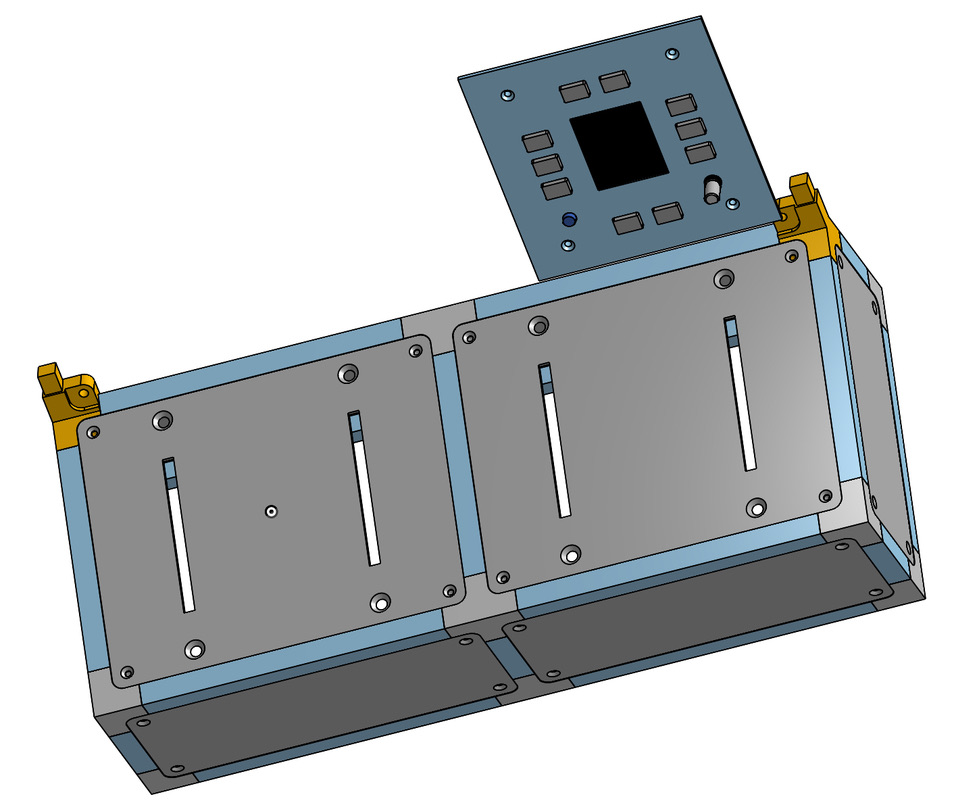
\includegraphics[scale=0.4]{images/EjemploEscritorio.jpeg}
    \caption{Ejemplo Escritorio Control}
    \label{fig:driverDeskExample}
\end{figure}
Figura 1 Ejemplo de panel en construccion
Este sistema tendrá que gestionar pantallas TFT, Palancas y Botones.

Como inspiración también se tiene la creación de cabinas personales de simulación de Avaviacion. En dicho hobby
se recrean cabinas muy realista, pero siempre se parte de la modularidad, esto es se divide en paneles
independientes, controlados cada uno con su arduino y este gestiona unos pocos botones/led para que sea realista.

En nuestro caso la idea es hacer diferentes paneles (TFT, Botones, dos o tres palancas,…) de tal forma que cada
uno se monte el panel como quiera y ajustado a sus necesidades.

Si no tenemos un protocolo de comunicaciones entre los paneles, necesitamos conectores específicos para cada tipo
de panel, por lo que el diseño de la placa central se complica y limita las posibilidades. Al añadir un protocolo
de comunicaciones podemos simplificar dicho diseño, pero implica un procesador por cada panel que transforme los
eventos del usuario a eventos del bus.

Así mismo no tiene sentido que cada panel se muestre al bus LCB emitiendo sus eventos y es mejor que se presente
al bus como un solo dispositivo y una placa central gestione cada panel.

\subsection{Problemas y Soluciones}
Además del problema obvio de pines (para capturar las pulsaciones de botones) el sistema inicial nos ha
identificado otros dos problemas, uno de ellos es la limitación de tiempo y coste de procesado, el otro es
la disponibilidad de librerías y/o periféricos.

\subsubsection{Detectar Pulsaciones}
El problema de capturar las pulsaciones de los botones de los usuarios es lineal, un botón -> un pin y ademas
nos interesa que sean interrupciones para que se capture la pulsación y no “haya” un coste computacional. Si no
son interrupciones debemos comprobar el estado del pin en cada bucle principal, pero esto implica que si el micro
procesador esta haciendo cosas largas, podamos perder pulsaciones por el usuario.

Las posibles soluciones son 4:
\begin{itemize}
    \item{} Uso de un procesador más poniente, con más pines e interrupciones.
    \item{} Matriz de MxN Keyboard  (\href{https://pcbheaven.com/wikipages/How_Key_Matrices_Works/}{How Key
              Matrices Works}) u otras variaciones basadas en resistencias/diodos. Esta solución require nos impide usar
          interrupciones y nos obliga a tener un bucle principal rápido y capturar el estado de los botones
    \item{} Usar un GPIO Expander o un chip de gestión de keyboard
    \item{} Usar un chip barato solo encargado de esto y usar un bus/protocolo propio
\end{itemize}

\subsubsection{Coste Computacional}
Ciertas operaciones requiren mucho tiempo de computación y si se realizan a la vez que el usuario interactúe con
el sistema es posible que se pierdan dichos eventos.

Por ejemplo el proceso de refrescar todos los leds WS2812 le lleva más de 100ms tiempo suficiente para que un
usuario pulse y libere un botón, si empezamos a añadir funciones, la ventana de oportunidad para detectar las
pulsaciones se reduce.

En este caso solo tenemos dos soluciones, o bien usamos un procesador más potente, bien usamos un procesador
para cada tarea intensiva.

\subsubsection{Disponibilidad de Librerías/Perifericos}
En el mercado existen diferentes micro-controladores que tienen periféricos diferentes como controladores CAN, % chktex 8
de LCD, WiFi, bluetooth y según las necesidad nos puede interesar usar uno u otro. En este caso de una forma u
otra deberemos acabar usando varios micro-controladores ya bien sea por usar varios con un bus controlado o con % chktex 8
chips dedicados y sus propios protocolos.

En este caso nos podemos encontrar con la (no) existencia de librerías para el micro elegido, con lo que usar
un bus propio nos permite tener chips que si nos lo soporte


\newpage{}
\section{Protocolo Base: I2C}
% !TeX encoding = UTF-8
% !TeX spellcheck = es_ES
% !TeX root = Proto.tex
%!TEX root=Proto.tex

Como base de nuestro Bus, vamos a utilizar I2C puesto que prácticamente todo los micro-controladores tienen % chktex 8
hardware dedicado para dicho protocolo y es el que menos pines nos requieren (2). SPI se descarta por requerir
mas pines (3+D). Dicho esto se ha evaluado y descartado los Buses CAN y RS-XXX por requerir como mínimo un chip % chktex 8
más (Transceivers o PHY) y no tendiendo todos los micros soporte a dichos buses. Estos buses, aun estando
pensados para realizar comunicaciones externas, es posible usarlos en cortas distancias, como una placa o entre
placas de un dispositivo cerrado.

Basandonos en el Modelo OSI de redes definiremos la capa física, I2C se encargara del transporte y la
comunicacion de los datos. Luego nos queda las capas superiores (sesión-aplicación) donde definiremos un % chktex 8
protocolo propio, uno base para poder gestionar los dispositivos y varios por encima para cada tipo de panel
que queramos hacer.

\subsection{Capa Fisica}
I2C ya nos marca unos mínimos de como deben ser las conexiones, en este apartado dejaremos simplemente la
definición de los conectores y los cables a usar.

La conexión física es en estrella, partiendo del nodo central o maestro. Pero todos los dispositivos compartiran
las lineas I2C (SDA y SCL)

Los cables serán AWG 22 e irán a un conector JST\_PH2.0 de 5 pines:

\begin{itemize}
    \item{} VCC (3.3v 100mA max)
    \item{} SDA (PullUp 1K Master)
    \item{} SCL (PullUp 1K Master)
    \item{} GND
    \item{} INT (PullUp 1K Master)
\end{itemize}


\subsection{Capa enlace}
En el caso de I2C los microcontroladores contienen hardware para gestionar el bus. En concreto el que hace de
master I2C. Este microcontrolador toma el control de las lineas I2C, tanto de SDA como SCL, (siendo esta ultima
el reloj para mandar y recivir datos). Como el Master controla el reloj, este debe saber cuando bytes va recibir.
Y el slave debe devolver ese mismo numero de bytes (sino los micro se bloquean)

Una trama fisica I2C tipica tiene la forma (Negro Controla Master, Rojo controla Slave):
\begin{figure}[H]
    \centering{}
    \begin{tikztimingtable}[
            scale=0.69,
            timing/dslope=0.1,
            timing/.style={x=4ex,y=2ex},
            x=1ex,
            timing/rowdist=5ex,
            timing/name/.style={font=\sffamily\scriptsize}
        ]
        SDA & L D{A6} D{A5} D{A4} D{A3} D{A2} D{A1} D{A0} D{R/W} D{[red]ACK} 8D{CMD} 8D{[red]Response}U \\
        SCL & h L 49{c} U \\
        \extracode()
        \begin{pgfonlayer}{background}
            \begin{scope}[semitransparent,semithick]
                \vertlines[darkgray,dotted]{2,6,...,106} % chktex 11
            \end{scope}
        \end{pgfonlayer}
    \end{tikztimingtable}
    \caption{Trama I2C de ejemplo}
    \label{fig:I2C Example}
\end{figure}

El bit R/W se supone que es para indicar si una operacion es de escritura o de lectura. Como en las librerias de
Arduino no se nos permite controlar este bit, no lo usaremos en el protocolo.

En codigo una peticion de un comando (CMD) que devuele una cantidad de bytes (SIZE) debe hacerse como:

\begin{mdCode}
    \lstset{language=C++,style=cppstyle}
    \begin{lstlisting}
Wire.beginTransmission(address);    // Iniciar comunicacion
Wire.write(CMD);                    // Enviar Commando
Wire.endTransmission(false);        // Preparar para response
Wire.requestFrom(address,SIZE);     // Solicitar response
while(Wire.available()>0){          // Tantas veces como SIZE
    byte slaveByte2 = Wire.read();  // Leer byte.
}
Wire.endTransmission(true);        // Liberar Bus
\end{lstlisting}
\end{mdCode}

Para nuestro protocolo base nos definiremos una trama de Request y una de Response. Ambas tramas constaran
de un byte cabecera incial y de otro final de CRC.\@

La cabecera en ambos casos contendra 6 bits para indicar un campo de Tamaño. Y los dos bits restantes para indicar
estados rapidos.

Por simplificar la funcion CRC sera la suma de todos los bytes haciendo un ``xor'' con la cadena  ``0xAA''.\@


\subsubsection{Trama Request}
La trama de request consta de 4 bytes, mas todos los bytes que el comando necesite para los parametros.

\begin{figure}[H]
    \centering{}
    \begin{bytefield}[bitformatting={\small\bfseries},
            bitwidth=2em,endianness=big]{8}
        \bitheader[]{0-7} \\ % chktex 8
        \begin{leftwordgroup}[]{Header}
            \bitbox{1}{\small Ext} & \bitbox{1}{\small R/W} & \bitbox{6}{R\_Size} % chktex 1
        \end{leftwordgroup} \\
        \bitbox{8}{Proto ID*} \\
        \bitbox{8}{CMD}\\
        \begin{leftwordgroup}[]{Parametros}
            \bitbox{8}{Params}\\
            \bitbox{8}{\dots}
        \end{leftwordgroup} \\
        \bitbox{8}{CRC}\\
    \end{bytefield}
    \caption{Trama Request}
    \label{fig:Request}
\end{figure}
Campos:
\begin{itemize}
    \item{} \textbf{Header}: cabecera de la peticion, con un par de flags y el tamaño de Respuesta.
          \begin{itemize}
              \item{} \textbf{Ext}: 1 Bit, Si esta habilitado la request sera de un Protocolo Extendido. Se debe
                    incluir el campo \textbf{Proto ID}
              \item{} \textbf{R/W}: 1 Bit, Identificador de tipo de request, ``Read'' o ``Write''. Como no podemos
                    controlar el bit I2C, lo ponemos aqui para asi poder indicarlo aqui. Asi nos permite utilizar estas tramas
                    sobre otros transportes.
              \item{} \textbf{R\_Size}: 6 Bits, Tamaño de la respuesta. Indica al cliente el numero de bytes que va a requerir el
                    Master. De esta forma el Dispositivo sabe cuantos bytes enviar. Al usar 6 bits nos permite indicar hasta 63 Bytes.
                    Se intentara indicar el numero exacto que la respuesta generara (\textbf{SHOULD} segun terminologia RFC)
          \end{itemize}
    \item{} \textbf{Proto ID}: Identificador del Protocolo de aplicacion, si el bit \textbf{Ext} es 0, la peticion
          es para un protocolo basico y este campo no debe enviarse.
    \item{} \textbf{CMD}: El identificador del Comando Requerido.
    \item{} \textbf{Params}: Los bytes que requiera el comando como parametros.
    \item{} \textbf{CRC}: Byte con el resultado de la funcion CRC segun se ha definido antes.
\end{itemize}

\subsubsection{Trama Response}
La respuesta a una request debe ser del mismo numero de bytes indicados en el campo \textbf{R\_Size} de
la misma, indistitanmente si los necesita o no. Para los casos que la respuesta no los necesite se debera incluir
tantos bytes de PAD como sea necesario para llenar el hueco. \textbf{R\_Size} incluye la cabecera y el CRC.\@
\begin{figure}[H]
    \centering{}
    \begin{bytefield}[bitformatting={\small\bfseries},
            bitwidth=2em,endianness=big]{8}
        \bitheader[]{0-7} \\ % chktex 8
        \begin{leftwordgroup}[]{R\_Size}
            \bitbox{1}[]{\small OF} & \bitbox{1}{\small Err} & \bitbox{6}{Size} \\ % chktex 1
            \begin{rightwordgroup}[]{Size}
                \bitbox{8}{Response} \\
                \bitbox{8}{\dots}
            \end{rightwordgroup}\\
            \bitbox{8}{PAD*} \\
            \bitbox{8}{\dots} \\
            \bitbox{8}{CRC}
        \end{leftwordgroup}
    \end{bytefield}
    \caption{Trama Response}
    \label{fig:Response}
\end{figure}

Campos:
\begin{itemize}
    \item{} \textbf{Header}: cabecera de la peticion, con un par de flags y el tamaño de Respuesta.
          \begin{itemize}
              \item{} \textbf{OF}: 1 Bit, Indica si los datos a responder no caben en tamaño asignado por \textbf{R\_Size}.
              \item{} \textbf{Err}: 1 Bit,  Indica si ha habido algun error. En caso afirmativo la respuesta sera un codigo de error
              \item{} \textbf{Size}: 6 Bits, Tamaño de la respuesta. Indica al Master cuantos bytes son realmente utiles, el resto seran
                    relleno
          \end{itemize}
    \item{} \textbf{Response}: Los Bytes con la respuesta. Si hay un error bit \textbf{Err} 1, sera el codigo de error.
    \item{} \textbf{PAD}: Bytes de relleno.
    \item{} \textbf{CRC}: Byte con el resultado de la funcion CRC segun se ha definido antes.
\end{itemize}

En el caso de que el tamaño solicitado sea insufciente para la respuesta, se debe crear una trama con los bits \textbf{OF} y \textbf{Err}
a 1 y la respuesta tendra codigo de error \textbf{REQUEST\_SIZE\_ERROR}\sidenote{Sea cual sea el valor
    definido, Mirar el anexo correspondiente}.

No obstante se puede dar el caso de que el dispositivo pueda responder parcialmente, ya que en el protocolo se tiene en cuenta el envio
y procesado de listas de elementos. El caso de que el cliente aun pueda responder con al menos un elemento la repuesta contendra el bit
\textbf{OF} a 1 pero \textbf{Err} a 0, esto es una indicacion de que se ha podido devolver parte de la informacion.

Como por ejemplo la la lista eventos del usuario. Se puede dar el caso de que el dispositivo tenga acumulados 10 eventos, pero la Request
de obtencion de eventos solo tenga hueco para 5. En este caso \textbf{Err} estara 0 y la response solo contendra 5 Eventos. El master
tendra que realizar otra request para obtener los 5 restantes.

El relleno o \textbf{PAD} son bytes sin informacion util pero si entran en el calculo del CRC.\@ Existen diferentes funciones para poner
un relleno, como un valor fijo, un patron conocido (FF00 \dots{} 00FF), \dots{}. Para este protocolo solo se exigira que todos los bytes
tengan el mismo valor y se recomienda que el valor sea el numero de bytes con relleno. En un futuro esto se podra comprobar.

\subsection{Protocolo Sesion}
Este protocolo sera el base que todos los dispositivos deben implementar, tendra funciones de
\begin{itemize}
    \item{} Init
    \item{} Reset
    \item{} Identificacion
    \item{} Gestion de direcciones I2C
    \item{} \dots{}
\end{itemize}

Por una parte se definiran el flujo para iniciar los dispositivos y una serie de Registros y Operaciones I2C para
el funcionamiento minimo de los dispostivos

\subsection{Protocolos de Aplicacion}

Por encima de I2C y de la sesion se definiran otros Registros/Operaciones I2C para cada uno de los tipos de
dispositivos que existan,  por ejemplo para botones, TFTs, palancas de control,\dots.


\newpage{}
\section{Capa Sesión}
% !TeX encoding = UTF-8
% !TeX spellcheck = es_ES
% !TeX root = Proto.tex
%!TEX root=Proto.tex
\subsection{Estados del dispositivo}
Un dispositivo tiene 5 estados tal y como se ve en el diagrama de estados:
\begin{figure}[H]
    \centering{}
    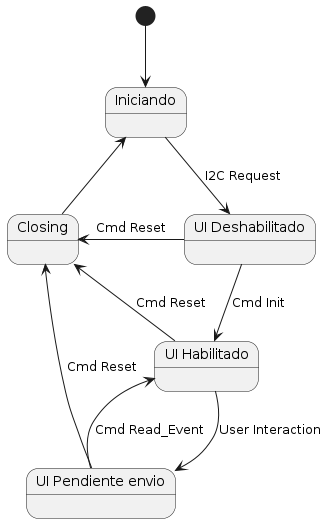
\includegraphics[scale=0.8]{images/states.png}
    \caption{Estados Dispositivos}
    \label{fig:deviceStates}
\end{figure}
En iniciando el dispositivo se acaba de iniciar (o de resetear) y esta a la espera de la primera request I2C.
En cuyo caso pasa a UI Deshabilitado, estado en el que el dispositivo respondera únicamente a peticiones I2C,
ignorando “todo” lo que haga el usuario.

Ante un comando de Iniciar, se pasa el estado UI Habilitado, en este estado se espera que el usuario realice
acciones (pulsar botón, mover palancas,…) y en cuanto se captura algun evento se pase a UI Pendiente de envio.
En este estado la línea INT debe estar baja. Cuando el máster envíe un comando de leer se vuelve a UI Habilitado
y se libera la linea INT.\\frac{}{}

Se espera que los eventos del usuario se gestionen en una Cola, por lo que UI Habilitado seria equivalente a
Cola Vacía  y UI Pendiente de envio Cola con Datos.

Una vez recivido el comando de reset el dispositivo se pasa a un estado de reseto donde puede hacer limpieza
de recursos antes de hacer un reset real. El proceso de limpieza debe terminar siempre y ejcutar una
interrupcion del procesador para hacer un reset.

Los dispositivos son libres de ampliar este diagrama de estados siempre y cuando ante el master respondan de
una manera coherente con este diagrama. Para ello se recomienda no ampliarlo y tener un segundo estado interno.

\subsection{Proceso de inicio}
El master a su vez ejecuta los siguientes pasos:
\begin{itemize}
    \item{} Lista los dispositivos I2C. (@, R, Stop), siguiendo los ejemplos “I2C scan”, el resultado es una lista
          de dispositivos (si podemos capturar el evento, el client bajara un pulso de su INT y registramos el pin INT)
    \item{} Para cada dispositivo ejecutara un proceso de identificación mandando varios comandos (ver seccion
          Identificacion) para comprobar que realmente es un dispositivo nuestro. En este
          paso detectaremos si hay algun conflicto (varios Dispositivos con la misma dirección I2C)
    \item{} Resolucion de conflictos (…)
    \item{} Inicializacion global (@=0)
\end{itemize}
A partir de este momento el master deberá estar mirando los pines de int y consultar el dispositivo cada vez que
este le baje a GND su linea de INT

\subsection{Identificación}
La identificación conlleva dos comandos, Obtener SN y Obtener Capacidades.

Las capacidades serán varios Bytes, siendo los primeros 6bits un identificador de tipo de panel (TFT, Botonera,….) 10 bits reservados para identificar hasta 10 protocolos básicos
(BTN, palancas, TFT,…) y luego bytes extra para incluir lista de protocolos soportados

Para cada protocolo se hará una consulta de capacidad a necesidad.

Luego estará el SN, que debe ser una cadena de bytes única para cualquier dipositivo, la idea es utilizar apis
de cada fabricante de microntrolador para usar el SN del dispositivo. Para que realmente sea único (por si
se da la casulidad de conflicto entre diferentes fabricantes) el primer byte sera un identificador de micro
(STM32, ATMEL, ESP32,…)



\newpage{}
\section{Anexo I: Comandos Protocolo Sesión}
% !TeX encoding = UTF-8
% !TeX spellcheck = es_ES
% !TeX root = Proto.tex
%!TEX root=Proto.tex

\begin{table}[h]
    \resizebox{\columnwidth}{!}{%
        \renewcommand\theadfont{\bfseries\sffamily}
        \begin{tabular}{|l|l|l|l|l|}
            \hline{}
            \thead{Comando}  & \thead{Codigo} & \thead{Parametros} & \thead{Respuesta}         & \thead{Condiciones}                                                                     \\ \hline{}
            Query I2C        & NA,R           &                    & ACK                       & Pulso Int si es posible                                                                 \\ \hline{}
            Get\_ID          & 0x01, R        &                    & Serial Number             &                                                                                         \\ \hline{}
            Get\_Caps        & 0x02, R        &                    & Capabilities              &                                                                                         \\ \hline{}
            Get\_Caps\_proto & 0x02, R        & ID\_Proto          & Capabilities\_proto       &                                                                                         \\ \hline{}
            Set\_addr        & 0x03, W        & nueva direccion    & OK/ERROR                  & Dirigida o Universal + Int\_down (solo uno)                                             \\ \hline{}
            get\_addr        & 0x03, R        &                    & direccion                 & \begin{tabular}[c]{@{}l@{}}Universal + Int\_down\\ Dirigida puede ser ping\end{tabular} \\ \hline{}
            reset            & 0x00,W         &                    & ACK                       & Dirigida o global                                                                       \\ \hline{}
            e\_stop          & 0x04,W         & boolean            & ACK                       & global                                                                                  \\ \hline{}
            sotd             & 0x05,W         &                    & ACK                       & global                                                                                  \\ \hline{}
            send\_int        & 0x06,W         &                    & ACK                       &                                                                                         \\ \hline{}
            ack\_int         & 0x06,R         &                    & Numero Eventos pendientes &                                                                                         \\ \hline{}
            read\_event      & 0x07,R         &                    & PrimerEvento              &                                                                                         \\ \hline{}
            Init             & 0x0F,W         &                    & ACK                       & Dirigida o Global                                                                       \\ \hline{}
            get\_status      & 0x0F,R         &                    & ID\_Estado                &                                                                                         \\ \hline{}
        \end{tabular}
    }
    \caption{Tabla de commandos}
    \label{tab:Commands}
\end{table}

\begin{itemize}
    \item{} Query\_I2c: Es la consulta de existencia de I2C, no tiene parámetros y es lo que usan los scanners I2C
          de ejemplo. Si es posible hará un pulso de la linea INT
    \item{} Get\_ID: obtiene el Número de Serie o identificador del dispositivo, sera un array de bytes
          no determinado, siendo el primero un identificador de tipo (fabricante u familia de microcontrolador)
          segido del serial number del silicio.
    \item{} get\_caps: Obtiene el byte array de las capacidades, 6 bits indincan el tipo panel y 10 bits los
          protocolos basicos soportados, luego tantos bytes como protocolos extra soporte.
    \item{} get\_caps\_proto: Se pasa como parámetro el id de protocolo y el dispositivo devuelve los bytes
          específicos de cada protocolo (como por ejemplo numero botones,…)
    \item{} set\_addr: Cambia la direccion I2C de un dispositivo, se necesita un reset despues. Puede ser dirigida
          o global, pero si es global la linea INT del dispositivo deberá estar bajo y SOLO uno en este estado.
    \item{} get\_addr: Lee la direccion de un disposivo, si es dirigido, es un ping y sirve para comprobar
          que entiende nuestro protocolo. Si es global solo responderá el dispositivo con la linea INT abajo y SOLO
          habrá uno.
    \item{} reset: Reinicia el dispositivo.
    \item{} e\_stop: señal de Parada, enviada desde el master. Por lo general sera la centralita quien lo lance
          ante un corto. Es una forma de avisar a los dispositivos el estado. Este commando tiene un parámetro binario
          con el estado del sistema.
    \item{} sotd: Start Of The Day. Señal para reloj Rápido, para indicar un comienzo del día.
    \item{} Send\_int, El master dirigira esta petición a un dispositivo con la idea de que el mismo baje su señal
          INT a GND. Se mantendrá bajo hasta que el máster mande un ack\_int o lea la última interrupción
    \item{} Ack\_int. El dispositivo destino devolverá el numero de eventos pendientes de leer, si es 0 liberará
          la linea INT
    \item{} Read\_event: El dispositivo destino devolverá al master el primer evento disponible, sera un array de
          bytes, donde el primer bytes identifica al protocolo y el resto de bytes serán dependiente del protocolo.
          Si la cola de enventos queda vacía liberarara la Linea INT
    \item{} Init: envía a los dispositivos la señal para avanzar de estado. Los dispositivos empezaran a aceptar
          los eventos de los usuarios.
    \item{} get\_status: El dispositivo devolverá un byte con el identificador del estado, según la tabla de
          estados definida en este protocolo.

\end{itemize}


\newpage{}
\section{Indice}
\tableofcontents{}

\listoffigures{}
\listoftables{}


\end{document}